\section{Collaborative Filtering}
In this section, two categories of methods involved in collaborative filtering that will be discussed: memory-based methods and model-based methods.
\subsection{Memory-Based Methods}
Collaborative filtering takes into account the fact that there is a relationship between the items and the user's preference. In memory-based approaches, as the name suggests, a memory-based recommender system typically needs to leverage the entire user-item dataset and make recommendations accordingly.
\begin{figure}[htbp]
\centering
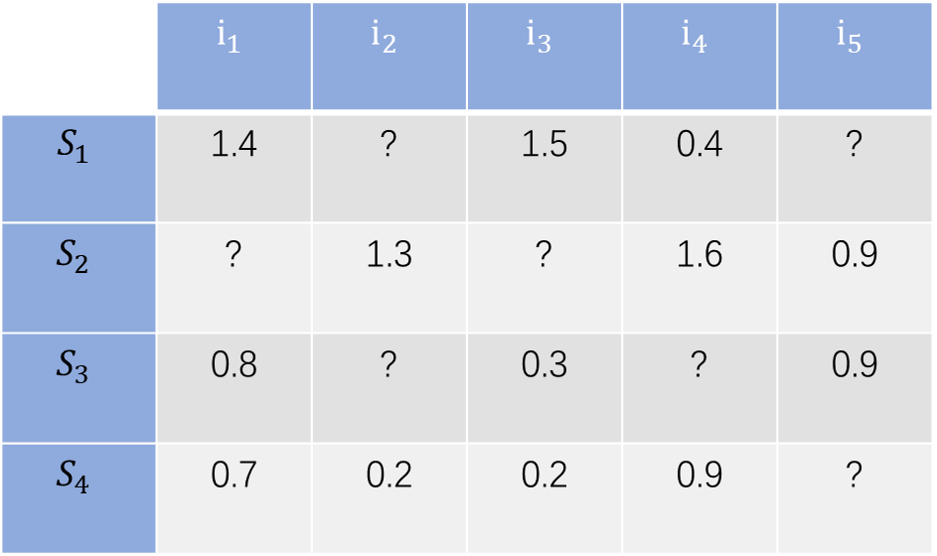
\includegraphics[scale=0.7]{figure/cf1.png}
%\caption{fig1}
\caption{User$-$item rating matrix}
\end{figure}
Once we have the user rating data for the items, we can convert them into the form of the matrix as shown in Figure 2.1. The horizontal coordinates are the users, and the vertical coordinates are the items. The corresponding number is the user's rating of the item. The question mark within the matrix indicates that the user has not rated the item, and our goal is to use collaborative filtering to predict unknown ratings. Memory-based collaborative filtering to make recommendations by similar users or similar items, then the question arises how to define similar users or similar items? The answer is similarity. After we have the user-item rating matrix, as shown above, the row vectors in the matrix represent the preferences of each user, and the column vectors represent the attributes of each item. This can be interpreted as meaning that there exists an attribute of the item that attracts users to provide a corresponding rating. So, by computing the similarity between row vectors, we will get the user similarity, and by computing the similarity of vertical vectors, the item similarity will get. \textit{Cosine similarity}, \textit{Pearson correlation coefficient}, and \textit{Euclidean distance} are the common methods to compute the similarity.

This chapter has demonstrated the concept of memory-based collaborative filtering. It is now necessary to explain the two basic approaches of memory-based collaborative filtering: the user-based method and the item-based method.
\subsubsection{User-Based Collaborative Filtering}
For user-based collaborative filtering, in each recommendation, we have a target user who will be recommended. The user-based collaborative filtering algorithm first identifies users that are similar to that particular target user, i.e., users that share the target user's rating pattern. User-based collaborative filtering predicated on similarities including history, preferences, and choices made by users when purchasing, viewing, or certain other behaviors. Based on the ability conferred by similarity, we can estimate the ratings that a target user might give based on similar users' ratings of items that the target user did not give a rating on. Based on the predicted rating, the user-based collaborative filtering algorithm can recommend items with higher ratings to the target users.
\begin{figure}
\centering
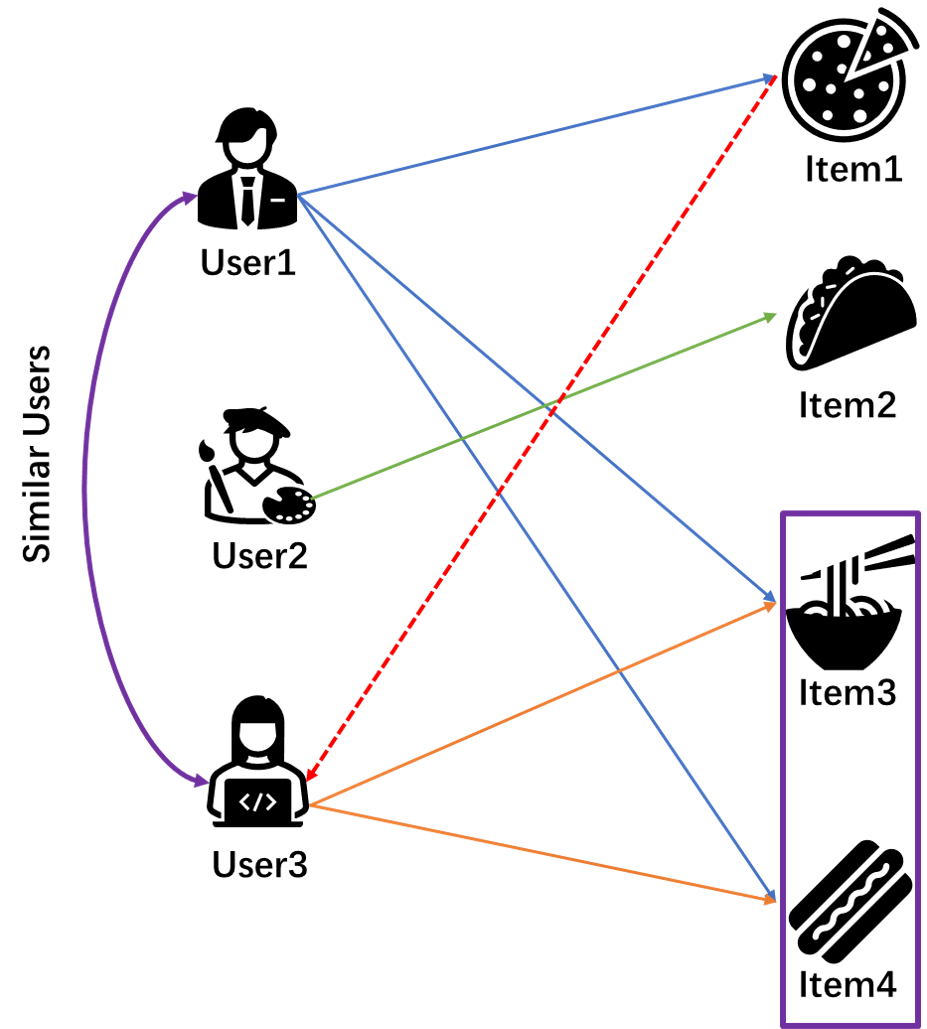
\includegraphics[scale=0.5]{figure/mo.png}
%\caption{fig1}
\caption{User-based collaborative filtering}
\end{figure}

User-based collaborative filtering can be illustrated briefly in Figure 2.2. Recall that the recommendation of the user-based method is based on similar users who share the same preference with the target user. As the example shown in Figure 2.2. Both \textit{user1} and \textit{user3} show a preference for \textit{item3} and \textit{item4}, and for this reason, we consider \textit{user1} and \textit{user3} to be similar users. Then, the user-based collaborative filtering algorithm will recommend \textit{item1} to \textit{user3} that \textit{item1} is the item that wins the positive rating by \textit{user3}’s similar user-\textit{user1}.

\subsubsection{Item-Based Collaborative Filtering}
Item-based collaborative filtering and user-based collaborative filtering are essentially the same. The only difference is that item-based collaborative filtering is based on the similarity between items instead of the similarity between users, as in user-based collaborative filtering. The idea of item-based collaborative filtering is to find items similar to those you have purchased or browsed, then recommend those items to you, i.e., ``Birds of a feather flock together."
\begin{figure}[htbp]
\centering
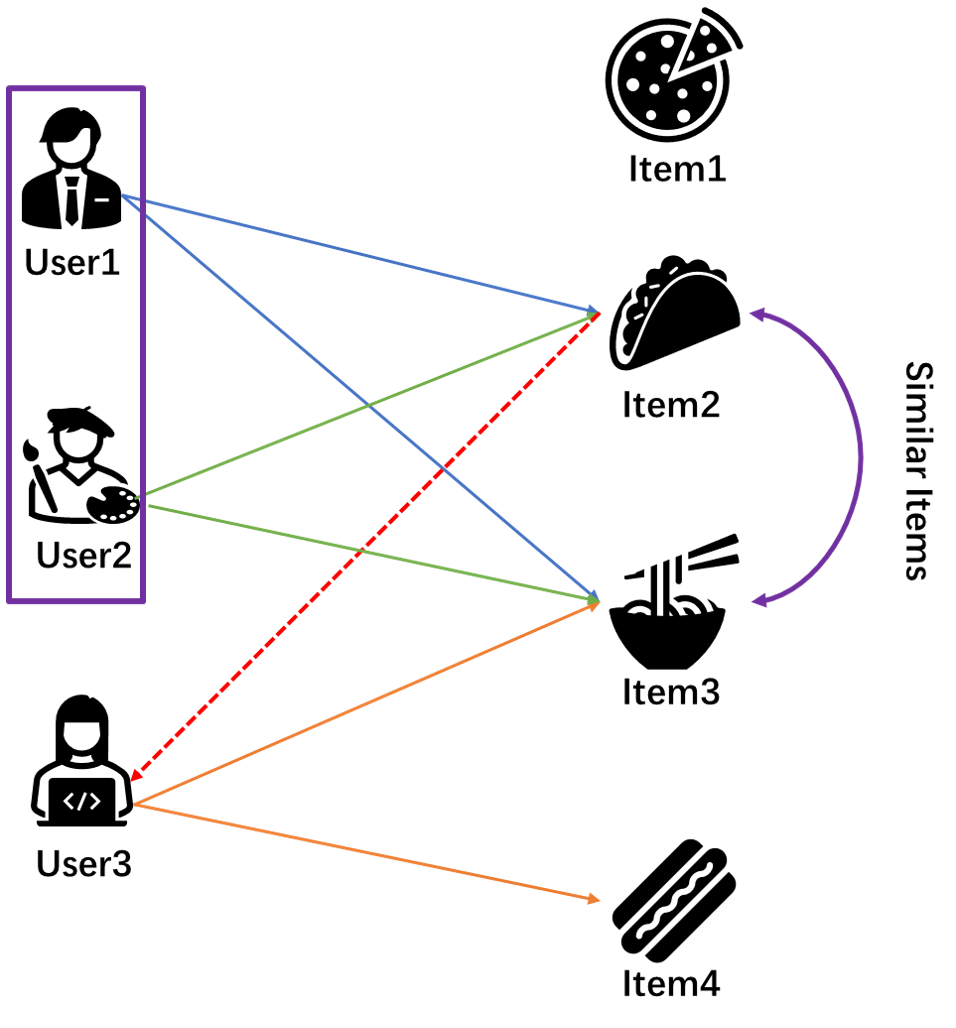
\includegraphics[scale=0.5]{figure/model2.png}
%\caption{fig1}
\caption{Item-based collaborative filtering}
\end{figure}

We use Figure 2.3 to interpret the process of item-based collaborative filtering. The first step is to identify the similar item through the behavior of users instead of the contents of the items ( if we use the content of the item as the similarity criterion, then the system will morph into a content-based recommendation system). In the example in Figure 2.3, \textit{item2} and \textit{item3} are regarded as similar items due to this two items were received a positive rating from both \textit{user1} and \textit{user2}. By the figure, we can see that \textit{user3} shows the preference on \textit{item3}, so the item-based collaborative filtering algorithm will choose \textit{item2} which is the similar item of \textit{item3} to recommend to the \textit{user3}.
\subsection{Model-Based Methods}
It is worth noting that in the real world, the number of users is generally huge (e.g., Netflix has millions of users), compared to the number and type of items that are relatively fixed. In this scenario, calculating the similarity between items offline by using item-based collaborative filtering is preferred in order to optimize the efficiency of recommendation. On the contrary, in the case of a small number of users, user-based collaborative filtering is preferred. It can be seen from this that there is no good or bad recommendation system, and the important thing is to choose the right recommendation method in the right situation.

As can be seen from the above, memory-based methods are intuitive and highly interpretable models. Users can easily figure out why the memory-based system recommends these items to them (due to their similar users preferring this item or the item is similar to the one you have purchased or viewed). But on the other hand, the effect of memory-based methods to recommend popular products is more obvious. That is to say, if a lot of people like \textit{item1}, under memory-based methods, the probability of recommending it to you will be higher, although if item \textit{item2} also matches your interest, due to the rating for \textit{item2} is sparse, so the similarity of item \textit{item2} is greatly reduced when calculating the similarity.

So, is there a method that can handle sparse data with better generalization ability? Turning now to the methods to address the above question, which are called model-based methods.
\subsubsection{Latent Factor Models}
Model-based collaborative filtering has been studied for decades, and many methods have been proposed. Such as in \cite{multifacetedcf}, a multifaceted collaborative filtering model has been proposed or the probabilistic matrix factorization be described in \cite{Probabilistic}. In general, model-based collaborative filtering can produce a more accurate recommendation \cite{multifacetedcf}. In this section, matrix factorization (MF) which is the most popular latent factor model, will be illustrated.

The purpose of matrix factorization is to discover latent factor models of users and items in a shared latent space where the user-item relationship (e.g., user rating of the item) is calculated from the inner product of the user matrix and the item matrix.For a user-item rating matrix \textit{R} consisting of $m$ users and $n$ items, where $R\in\mathbb{R}^{m\times n}$. Through matrix factorization, the $m\times n$ user-item matrix \textit{R} be factorized into user latent matrix \textit{p} ($m\times k$ matrix) and item latent matrix \textit{q} ($k\times n$ matrix), where \textit{k} is the dimension of the \textit{latent factor}. In matrix factorization, the latent model of user \textit{u} and item \textit{i} are denoted by $p_{u}$ and $q_{i}$ respectively, where $p_{u} \in\mathbb{R}^{k}$, $q_{i} \in\mathbb{R}^{k}$. The notation ${r}_{u,i}$ is used to represent the rating of user \textit{u} on item \textit{i}. The predicted rating of user \textit{u} on item \textit{i} can be described as :
\begin{equation}
    \hat{r}_{u,i}=q_{i}^{T}p_{u}
\end{equation}
A general approach to training the latent model is to minimize the gap between predicted rating $\hat{r}_{u,i}$ and real rating $r_{u,i}$ that can be express as ${r}_{u,i}-q_{i}^{T}p_{u}$, by adopting \textit{root mean square error} (RMSE) as the loss function, we have:
    \begin{equation}
        \operatorname{Loss}=\min_{ q *, p * }\sum_{(u, i) \in K}\left(r_{u,i}-q_{i}^{T} p_{u}\right)^{2}
    \end{equation}
where $K$ denotes the set of $(u,i)$ pairs. By adopting $\mathit{l}_{2}$ regularization to void over-fitting problem, we have:
    \begin{equation}
        \operatorname{Loss}=\min_{ q *, p * }\sum_{(u, i) \in K}\left(r_{u, i}-q_{i}^{T} p_{u}\right)^{2}+\lambda\left(\left\|q_{i}\right\|+\left\|p_{u}\right\|\right)^{2}
    \end{equation}